\chapter{Obtención, procesado y almacenamiento de los datos} \label{ch: dataGathering}
En este capítulo se abarca cómo se han obtenido los datos, cómo han sido almacenados y preprocesados para su explotación.

Los datos de conversaciones limpias de ruido no son algo fácil de conseguir. Son archivos que ocupan mucho disco y no se encontraron repositorios con la cantidad de información necesaria. Por otro lado está la obtención de ruidos, esta tarea si es más sencilla dado que existe gran diversidad de formas de descargarlos para sumarlos con los audios libres de ruido.

\section{Audio}
En primer lugar cabe destacar que se tuvieron en cuenta varias posibilidades durante dicha fase. A continuación se describen haciendo hincapié en la opción elegida.

\subsection{Extracción audio de YouTube}
La primera opción que se tuvo en cuenta fue la extracción del audio de videos alojados en \textbf{YouTube} de entrevistas y programas radiofónicos. Este tipo de fuentes conlleva el problema de que no se sabe a priori cuánto libres de ruidos están los audios. Usualmente, se introducen efectos o el ruido del público puede interferir el entrenamiento. Para evitar este problema habría que analizar todos los audios descargados, tarea tediosa y que requiere mucho tiempo.

\subsection{Generación de audio sintético}
La segunda opción que se barajó fue la generación de audio sintético. La generación de datos sintéticos es una técnica muy usada en el entrenamiento de modelos de \gls{ML}. Existen dos grupos en la generación de datos sintéticos:
\begin{itemize}
	\item \textbf{A partir de datos existentes}. Estas técnicas son muy usadas en el análisis de imágenes. Es muy típico ampliar el \MakeLowercase{\gls{dataset}} de imágenes para clasificadores aplicando transformaciones a la imágenes. Por ejemplo, si se está diseñando un clasificador de tipos de imágenes, una forma de ampliar el \gls{dataset} sería generar imágenes espejo de la originales. Esto consiste simplemente ordenar las columnas de la matriz de forma opuesta.
	\item \textbf{Desde cero}. Estas técnicas requieren usualmente de una red neuronal o algoritmo previamente entrenada que sea capaz de generar dichos datos de manera que sean prácticamente igual a unos reales.
\end{itemize}

En el caso del audio no se puede partir de un audio para modificarlo y expandir el \gls{dataset}. La única forma sería aplicar una ganancia en cuyo caso sería igual a subir o bajar el volumen, pero no es técnicamente generar datos nuevos. Por esta razón se eligió la segunda forma de generar datos sintéticos.

En el caso del audio los sintetizadores existen hace mucho tiempo. Los dispositivos \gls{GPS} de los automóviles tiene un sintetizador que reproduce una voz hablada. Estos sintetizadores son algo realmente complicado de hacer y típicamente tienen voces metálicas que no reproducen fielmente una voz humana. De hecho este es un gran campo dentro de las redes neuronales profundas. Estos tipos de algoritmo se denominan \textit{text to speech}.

Para este trabajo se desplegó el algoritmo \textit{\href{https://github.com/CorentinJ/Real-Time-Voice-Cloning}{Real Time Voice Cloning}}. Este algoritmo es un proyecto de código abierto que consiste en una red neuronal para la clonación de voz\cite{transfer_learning}. El algoritmo se entrena con una voz y después es capaz de reproducir audio con dicha voz a partir de texto.

Finalmente, tras un breve entrenamiento de esta red, se descartó debido a que lo resultados generaban una voz metálica. Esto es debido al corto entrenamiento al que fue sometida la red. Cabe destacar que es un algoritmo costoso que, corriendo en gráfica dedicada tarda en generar el audio pero es un algoritmo con gran futuro y fuertemente apoyado por la comunidad open-source.

\subsection{Descarga masiva de audiolibros}
Los audiolibros son una fuente de audio en la cual no deben existir ruidos externos que afecten a la grabación, adicionalmente, son grabaciones reales de personas y se tiene mucha información adicional como el texto que se está leyendo. Por estas razones son fuentes muy válidas para entrenar redes neuronales relacionadas con el análisis de la voz humana.

Como contrapartida está que la mayoría de los audiolibros son de pago y no están disponibles para una descarga masiva. Afortunadamente, existen diferentes sitios web que almacenan audios libros de dominio público, una de las más conocidas es \href{https://librivox.org/}{Librivox}. Esta web posee audiolibros en varios idiomas perfectamente clasificados y con gran cantidad de información sobre los mismo. Adicionalmente, cuenta con una \gls{API} que consiste en un servicio web que recibe peticiones \gls{GET} y devuelve en formato \gls{HTML} o \gls{JSON} la información solicitada. Este servicio web fue probado pero los resultados no fueron los esperados dado que cuando se aplicaban los filtros, la información devuelta por el servicio no cumplía las restricciones impuestas. Como consecuencia se descartó este método de obtención de la información y las \glspl{URL} de descarga de los libros. En su lugar, se planteó el desarrollo de un algoritmo de \gls{scraper}.

Los algoritmos de \gls{scraper} son altamente utilizados para la extracción de información de manera masiva y automatizada de los sitios web. Cuando se hace una petición a un sitio web éste devuelve el código de la página web que está almacenado en el servidor que proporciona el servicio de almacenamiento web, en inglés, \textit{hosting} y el navegador web lo interpreta mostrando su contenido. La figura \ref{fig: web_nav} presenta un esquema resumido de esta comunicación. Este código puede ser analizado por un algoritmo para extraer información, salvo que el código de la página haya sido ofuscado, dado que es un código altamente estructurado. Este tipo de técnicas están en la frontera de la ética dado que también pueden ser usadas para hackeo web.

\begin{figure}[ht!]
	\centering
	\resizebox{!}{!}{
		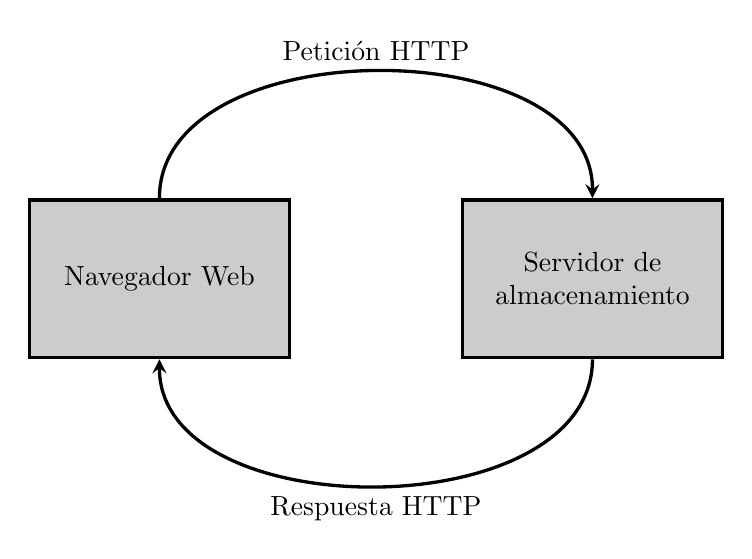
\begin{tikzpicture}
		\tikzstyle{box} = [draw,inner sep=7,minimum size=57,line 
		width=1, very thick, draw=black, fill=black!20, text width=80, text centered]
		\tikzstyle{invisible} = [outer sep=0,inner sep=0,minimum size=0]
		\tikzstyle{stealth} = [-stealth]
		\node [box] (v1) at (0,0) {Navegador Web};
		\node [box] (v2) at (5.5,0) {Servidor de almacenamiento};
		
		\draw [stealth, in=90, out=90, very thick] (v1) edge node [anchor=south] {Petición HTTP}(v2);
		\draw [stealth, in=270, out=270, very thick] (v2) edge node [anchor=north] {Respuesta HTTP} (v1);
		\end{tikzpicture}
	}      
	\caption{Esquema de la navegación web}
	\label{fig: web_nav}
\end{figure}

Las técnias de \gls{scraper} están compuestas por varios pasos:
\begin{itemize}
	\item Exploración visual del sitio web.
	\item Análisis de la \gls{URL}. En muchas ocasiones, parte de la información que el sitio web devuelve viene filtrada mediante una serie de filtros que se definen en la \gls{URL}.
	\item Análisis del sitio web mediante herramientas de desarrollador. Consiste analizar el sitio web para encontrar dónde está la información que se quiere extraer y cómo viene en el código de la página. Para esto se usa un navegador web y se analiza el código mediante el inspector del navegador. Esta herramienta resalta cada una de las partes del código de la página web que se corresponden con las partes visuales de la misma.
	\item Extracción y almacenamiento de la información.
\end{itemize}

Existen dos tipos principales de \gls{scraper} en función del tipo de web a la que se le quiera extraer la información y del tipo de seguridad que lleve implementada:
\begin{itemize}
	\item Sitios web estáticos. Extracción con peticiones librerías de peticiones web y respuestas en código \gls{HTML}
	\item Sitio web dinámicos. Extracción avanzado mediante un driver de navegador (Firefox, Chrome\dots) y respuestas de código JavaScript.
\end{itemize}
El primero de los tipos consiste en hacer peticiones a la \gls{URL} objetivo y extraer la información devuelta en la petición. Este tipo de algoritmos no permiten hacer una navegación interactiva por la página y no permite interactuar con JavaScript, algo cada vez más presenta en las webs actuales. Como punto a favor, estos tipos de algoritmo son muy rápidos y fáciles de desarrollar. En contra partida, si se hace un número grande de peticiones al servidor éste puede bloquear la IP de entrada de la petición para protegerse a ataques.

El segundo tipo consiste en la emulación de la navegación humana llamando al navegador. Estas técnicas son mucho más avanzadas y permiten obtener información de cualquier página, rellenar formularios y hacer uso de la página como si de un humano se tratara. Aporta muchas más posibilidades que el otro tipo de \gls{scraper} y es mucho más robusto y bloqueos por parte del servidor, esto se puede mejorar incluso, poniendo esperas aleatorias entre peticiones. Sin embargo, ejecuta un navegador y, por consiguiente, es mucho más lenta la extracción de la información.

\subsubsection{Exploración visual}
Para el caso concreta del trabajo, la web objetivo se puede ver que contiene diferentes formas de analizar el catálogo. Esto no son más que filtros que se le pueden aplicar a la base de datos donde la página almacena la información. En la figura \ref{fig: librivox_cover} se puede ver la estructura de la página.
\begin{figure}[ht!]
	\centering
	\resizebox{\textwidth}{!}{
		\includegraphics[width=\columnwidth]{figures/LibriVox_cover.png}
	}      
	\caption{LibriVox página principal}
	\label{fig: librivox_cover}
\end{figure}
\subsubsection{Análisis de la \acrshort{URL}}
A continuación se selecciona el filtro del lenguaje puesto que el trabajo se va a entrar para audiolibros en castellano. El navegador se actualiza y muestra el siguiente contenido en la barra de dirección.
\begin{center}
	\fbox{%
	\tiny{https://librivox.org/search?primary\_key=5\&search\_category=language\&search\_page=1\&search\_form=get\_results}
	}%
\end{center}
De esta información se pueden extraer que existen varios tipos de información separados por el caracter \textbf{\&} organizados como \textbf{atributo=valor}. A continuación se analizan cada uno de los filtros:
\begin{itemize}
	\item \textbf{primary\_key} es el valor del campo principal de búsqueda, en este paso como se busca por la categoría \textbf{language} el valor \textbf{5} representa el \textbf{español}.
	\item \textbf{search\_category} esta campo representa la categoría mediante la cual se están haciendo la búsqueda. Otros posibles valores serían \textbf{author}, \textbf{title}, entre otros.
	\item \textbf{search\_page} este campo representa la página actual de búsqueda. Por consiguiente para cambiar de página dentro del mismo idioma se debe ir incrementando este número
\end{itemize}
\subsubsection{Análisis del sitio web con herramientas de desarrollador}
El siguiente paso consiste en analizar cómo están la información en la paǵina web. En este caso, la lista de resultados la devuelve un JavaScript que tarda unos segundos en cargar. Después de la carga se puede empezar a analizar el contenido como muestra la figura \ref{fig: librivox_inspect}
\begin{figure}[ht!]
	\centering
	\resizebox{\textwidth}{!}{
		\includegraphics[width=\columnwidth]{figures/LibriVox_inspect.png}
	}      
	\caption{LibriVox analizado con el inspector de Firefox}
	\label{fig: librivox_inspect}
\end{figure}

\begin{lstlisting}[style=HTML,basicstyle=\tiny\ttfamily, caption={Ejemplo de la información contenida para uno de los libros},captionpos=b, label={lst: librivox_book}]
<li class="catalog-result">
  <a href="#" class="book-cover">
    <img src="https://archive.org/download/thumbs_02/cien_mejores_1502_thumb.jpg"
       alt="book-cover-65x65" width="65" height="65">
  </a>
  <div class="result-data">
    <h3>
    <a href="https://librivox.org/las-cien-mejores-poesias-de-la-lengua-castellana-by-marcelino-menendez-y-pelayo/">
      A buen juez mejor testigo (in Las Cien Mejores Poesías de la Lengua Castellana )
    </a></h3>
    <p class="book-author"> <a href="https://librivox.org/author/11155">José ZORRILLA Y MORAL (1817 - 1893)</a> </p>
    <p class="book-meta"> Complete | Collaborative | Spanish</p>
  </div>	
  <div class="download-btn">
    <a href="http://www.archive.org/download//100mejorespoesias_1502_librivox/100mejorespoesias_1502_librivox_64kb_mp3.zip">
      Download
    </a>
    <span>248MB</span>
  </div>
</li>
\end{lstlisting}
Los datos de los libros que devuelve la búsqueda para dicha página se encuentran dentro de los bloques \textcolor{editorBlue}{$<$}\textcolor{editorPink}{li class}\textcolor{editorBlue}{=}\textcolor{editorPurple}{''catalog-result''}\textcolor{editorBlue}{$>$}. El ejemplo del contenido de uno de ellos se encuentra en el listado de código \ref{lst: librivox_book}. Se puede ver que hay mucha información sobre el libro, inclusive, la \gls{URL} de descarga del mismo.
\subsubsection{Extracción y almacenamiento de la información}
Para la extracción de la información se desarrolló un algoritmo basado en un webdriver con la librería de \textit{Selenium} y en el parseador de \gls{HTML} \textit{BeautifulSoup}. El algoritmo consiste en ir incrementando el valor de página y buscando toda la información de los libros en dicha página después de que la Query haya cargado. Para esto se busca el valor de la última página; si este valor es nulo, se incrementa un segundo el tiempo aleatorio de espera para el parseo de los datos. Si el valor obtenido es distinto de nulo, significa que la página ha cargado, entonces, se parsea la información de todos los libros en la página y se almacena en una base de datos \textit{SQLite}. En la figura \ref{fig: librivox_scraper_flowchart} se puede ver el diagrama de flujo del código para la parte del scraper y en \ref{lst: librivox_scraper} se puede ver el código que implementa la clase.

\begin{figure}[ht!]
	\centering
	\resizebox{!}{0.8\textheight}{
		\begin{tikzpicture}
		\tikzstyle{box} = [draw,inner sep=7,minimum size=57,line 
		width=1, very thick, draw=black, fill=black!20, text width=120, text centered]
		\tikzstyle{invisible} = [outer sep=0,inner sep=0,minimum size=0]
		\tikzstyle{stealth} = [-stealth]
		
		\tikzstyle{decision} = [diamond, draw, fill=yellow!20, 
		text width=6em, text badly centered, node distance=3cm, inner sep=0pt]
		\tikzstyle{block} = [rectangle, draw, fill=gray!20, 
		text width=12em, text centered, rounded corners, minimum height=4em]
		\tikzstyle{small_block} = [circle, draw, fill=white!20, 
		text width=0em, text centered, rounded corners, minimum height=0em]    
		\tikzstyle{cloud} = [draw, ellipse,fill=red!20, node distance=3cm,
		minimum height=2em]
		
		\node [cloud] (v8) at (0,3.5) {\textbf{Start}};
		\node [block] (v3) at (0,1.5) {\vspace*{-0pt}\begin{itemize}
			\item lastPage=0 \vspace*{-0pt}
			\item increaseSleep=0 \vspace*{-0pt}
			\item page=1 \vspace*{-0pt}
			\item availablePage=True
			\end{itemize}};
		\node [block] (v2) at (0,-1) {Update URL\\ GET URL};
		\node [block] (v4) at (0,-3) {Sleep[random(0.5,1) + increaseSlepp]};
		\node [block] (v5) at (0,-5) {Parse lastPageNode};
		\node [decision] (v6) at (0,-8) {lastPageNode == Null?};
		\node [block] (v1) at (-3.5,-10) {increaseSleep+=1};
		\node [block] (v7) at (3.5,-10) {increaseSleep=0};
		\draw [stealth,out=180,in=180] (v1) edge (v2);
		\draw [stealth] (v3) edge (v2);
		\draw [stealth] (v2) edge (v4);
		\draw [stealth] (v4) edge (v5);
		\draw [stealth] (v5) edge (v6);
		\draw [stealth,out=180,in=90] (v6) edge node[anchor=east]{YES} (v1);
		\draw [stealth,out=0,in=90] (v6) edge node[anchor=west]{NO} (v7);
		\draw [stealth] (v8) edge (v3);
		\node [decision] (v9) at (3.5,-13) {lastPage == 0?};
		\node [block] (v10) at (-1,-14.5) {Update lastPage val(lastPageNode)};
		\draw [stealth,out=180,in=90] (v9) edge node [anchor=south east]{YES} (v10);
		\node [block] (v13) at (3.5,-16.5) {Parse information for every book in the query};
		\node [block] (v12) at (-1,-21) {page+=1};
		\node [decision] (v11) at (3.5,-19.5) {page == lastPage?};
		\draw [stealth,out=180,in=90] (v11) edge  node [anchor=south east]{NO} (v12);
		\draw [stealth,out=180,in=180] (v12) edge (v2);
		\draw [stealth] (v9) edge node [anchor=south east]{NO} (v13);
		\draw [stealth] (v7) edge (v9);
		\draw [stealth] (v13) edge (v11);
		\draw [stealth,out=270,in=180] (v10) edge (v13);
		\node [cloud] (v14) at (5.5,-21) {\textbf{end}};
		\draw [stealth,out=0,in=90] (v11) edge node[anchor=west]{YES} (v14);
		\end{tikzpicture}
	}      
	\caption{Diagrama de flujo para el scraper de LibriVox}
	\label{fig: librivox_scraper_flowchart}
\end{figure}

\section{Ruido}
Para el ruido se han seleccionado vídeos de YouTube con ruidos urbanos, murmullo, lluvia y ruido característico de un centro de procesado de datos. Estos vídeos se han descargado mediante la librería \textit{youtube\_dl} y se les ha extraído el sonido así como información referente a la tasa de muestro, duración y el número de canales. Esta información junto con la localización de almacenamiento se ha introducido en la base de datos de SQLite. En \ref{lst: noise_manager} se puede ver el código que implementa esta parte del proyecto.
